% !TEX root = ../../../main.tex
% 来源：中学数学实验教材·第一册（代数）
% 章节：因式分解与余式定理 / 辗转相除法
% 原始文件：5.tex，行 2585-2607
% 类型：tikz
% ---
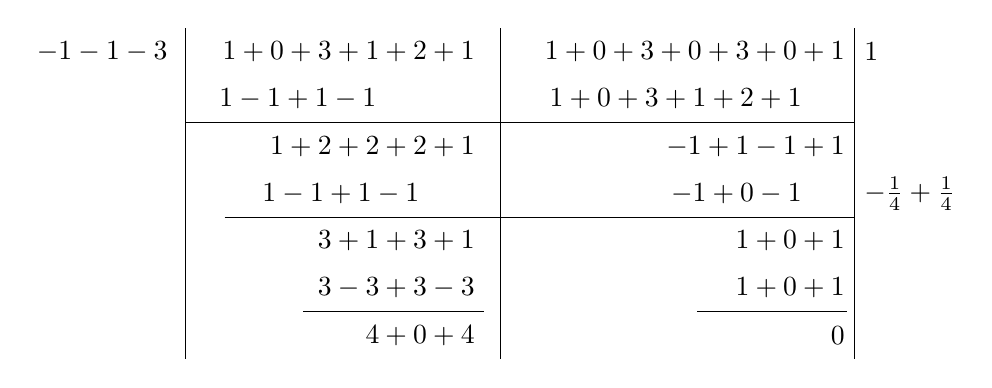
\begin{tikzpicture}[yscale=.6]
\foreach \y/\ytext in {6/1+0+3+1+2+1   ,5/1-1+1-1\qquad\quad\;\;   ,4/1+2+2+2+1  ,3/ 1-1+1-1\qquad   , 2/ 3+1+3+1 , 1/3-3+3-3, 0/4+0+4 }
{
    \node at (-.2,\y)[left]{$\ytext$};
}

\foreach \y/\ytext in {6/1+0+3+0+3+0+1  ,5/1+0+3+1+2+1\quad\;\;  ,4/ -1+1-1+1  , 3/ -1+0-1\quad\;\;   , 2/1+0+1, 1/1+0+1, 0/0}
{
    \node at (4.5,\y)[left]{$\ytext$};
}
\foreach \x in {-4,0,4.5}
{
    \draw(\x,6.5)--(\x, -.5);
}

\draw(-4,4.5)--(4.5,4.5);
\draw(-3.5,2.5)--(4.5,2.5);
\draw(-2.5,.5)--(-.2,.5);
\draw(2.5,.5)--(4.4,.5);
\node at (-4.1,6)[left]{$-1-1-3$};
\node at (4.5,3)[right]{$-\frac{1}{4}+\frac{1}{4}$};
\node at (4.5,6)[right]{$1$};
\end{tikzpicture}
